\chapter{原子核平均场及多核子组态}

\section{原子核平均场}
\paragraph*{平均场近似:}
\begin{enumerate}
	\item 质量数$A$,质子数$Z$,中子数$N$,满足$A=N+Z$;
	\item 核子间有强相互作用(核力),特别的,质子直接按
	\item 把核子当成没有内部结构的点粒子;
\end{enumerate}

\paragraph*{原子核集体波函数$\Psi_0$的理解:}在\uline{\textsl{Hartree}}方法中,集体波函数只表现为单粒子态的直积形式,如下
\begin{equation}
	\Psi_0(\bm{r}_1,\ \bm{r}_2,\ \bm{r}_3,\cdots,\ \bm{r}_A) = \prod_{i=1}^{A} \phi_{\alpha_i}(\bm{r}_i)
\end{equation} 
在\uline{\textsl{Hartree-Fock}}方法中,集体波函数表现为有个单粒子直积形式的混合,且具有反对称性质,如下
\begin{equation}
    \begin{aligned}
		\Psi_0(\bm{r}_1, \bm{r}_2, \bm{r}_3, \cdots, \bm{r}_A) ={}& \mathcal{A}\left[ \prod_{i=1}^{A} \phi_{\alpha_i}(\bm{r}_i) \right]	\\
		={}& 
		\begin{vmatrix}
			\phi_1(\bm{r}_1)	&	\phi_1(\bm{r}_2)	&	\phi_1(\bm{r}_3)	&	\cdots	&	\phi_1(\bm{r}_A)	\\
			\phi_2(\bm{r}_1)	&	\phi_2(\bm{r}_2)	&	\phi_2(\bm{r}_3)	&	\cdots	&	\phi_2(\bm{r}_A)	\\
			\phi_3(\bm{r}_1)	&	\phi_3(\bm{r}_2)	&	\phi_3(\bm{r}_3)	&	\cdots	&	\phi_3(\bm{r}_A)	\\
			\vdots				&	\vdots				&	\vdots				&	\ddots	&	\vdots				\\
			\phi_A(\bm{r}_1)	&	\phi_A(\bm{r}_2)	&	\phi_A(\bm{r}_3)	&	\cdots	&	\phi_A(\bm{r}_A)	\\
		\end{vmatrix}
    \end{aligned}
\end{equation} 
	其中,$\mathcal{A}$为反对称化算符,并且包含了归一化系数;$\bm{r}_1,\ \bm{r}_2,\ \cdots,\ \bm{r}_A$表示粒子$1,\ 2,\ \cdots,\ A$的坐标;$\phi_1,\ \phi_2,\ \cdots,\ \phi_A$表示有那么多个能级,也就是粒子可能占据的能级。我们现在考虑三粒子体系的情况,三个粒子占据三个能级,在\textsl{Hartree-Fock}方法中,其集体波函数可表示为
\begin{equation}
    \begin{aligned}
		\Psi_0(\bm{r}_1, \bm{r}_2, \bm{r}_3) ={}& \mathcal{A}\left[ \prod_{i=1}^{3} \phi_{\alpha_i}(\bm{r}_i) \right]	\\
		={}& \frac{1}{\sqrt{6}} 
		\begin{vmatrix}
			\phi_1(\bm{r}_1)	&	\phi_1(\bm{r}_2)	&	\phi_1(\bm{r}_3)	\\
			\phi_2(\bm{r}_1)	&	\phi_2(\bm{r}_2)	&	\phi_2(\bm{r}_3)	\\
			\phi_3(\bm{r}_1)	&	\phi_3(\bm{r}_2)	&	\phi_3(\bm{r}_3)	\\
		\end{vmatrix}	\\
		={}& \phi_1(\bm{r}_1)\phi_2(\bm{r}_2)\phi_3(\bm{r}_3) + \phi_1(\bm{r}_2)\phi_2(\bm{r}_3)\phi_3(\bm{r}_1) + \phi_1(\bm{r}_3)\phi_2(\bm{r}_1)\phi_3(\bm{r}_2) \\
		&- \phi_1(\bm{r}_3)\phi_2(\bm{r}_2)\phi_3(\bm{r}_1) - \phi_1(\bm{r}_2)\phi_2(\bm{r}_1)\phi_3(\bm{r}_3) - \phi_1(\bm{r}_1)\phi_2(\bm{r}_3)\phi_3(\bm{r}_2) 
    \end{aligned}
\end{equation} 
现在我们考察上式第二个等号的左边第一项,$\phi_1(\bm{r}_1)\phi_2(\bm{r}_2)\phi_3(\bm{r}_3)$表示粒子$1$处于能级$\phi_1$、位置在$\bm{r}_1$,且粒子$2$处于能级$\phi_2$、位置在$\bm{r}_2$,同时粒子$3$处于能级$\phi_3$、位置在$\bm{r}_3$的概率;后面几项类同。事实上,由于全同粒子的不可区分性,我们根本无法辨别粒子$1$、$2$、$3$,因此我们无法判断具体某一个态上的粒子具体是$1$、$2$、$3$中的哪一个,所以我们需要把各种情况考虑进来,同时考虑费米子的交换反对称性应加上对应的相位,上式最后一个等号右边的排列情况构成了如图\ref{fig:three-body-wv}所示:
\begin{figure}[htbp]
	\centering
	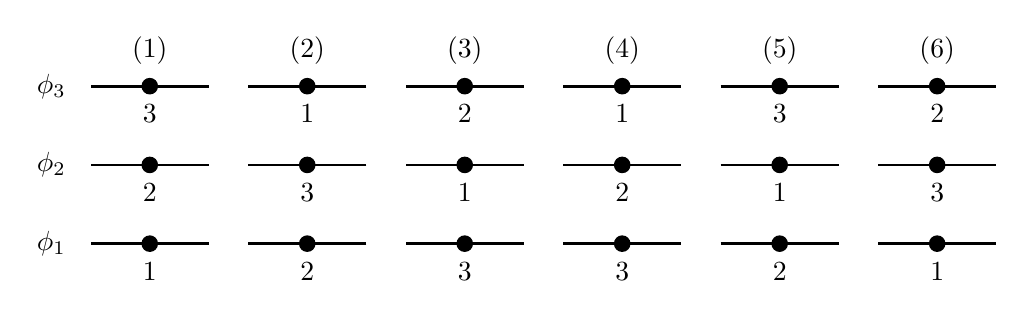
\begin{tikzpicture}
		\node at (-6.25, 2) {$\phi_3$};
		\node at (-6.25, 1) {$\phi_2$};
		\node at (-6.25, 0) {$\phi_1$};

		\node at (-5, 2.45) {(1)};
		\draw[line width=1pt] (-4.25, 2) -- (-5.75, 2);
		\draw[line width=1pt] (-4.25, 1) -- (-5.75, 1);
		\draw[line width=1pt] (-4.25, 0) -- (-5.75, 0);
		\fill (-5, 0)circle(3pt) (-5, 1)circle(3pt) (-5, 2)circle(3pt);
		\node at (-5, -0.35) {$1$};
		\node at (-5,  0.65) {$2$};
		\node at (-5,  1.65) {$3$};

		\node at (-3, 2.45) {(2)};
		\draw[line width=1pt] (-2.25, 2) -- (-3.75, 2);
		\draw[line width=1pt] (-2.25, 1) -- (-3.75, 1);
		\draw[line width=1pt] (-2.25, 0) -- (-3.75, 0);
		\fill (-3, 0)circle(3pt) (-3, 1)circle(3pt) (-3, 2)circle(3pt);
		\node at (-3, -0.35) {$2$};
		\node at (-3,  0.65) {$3$};
		\node at (-3,  1.65) {$1$};

		\node at (-1, 2.45) {(3)};
		\draw[line width=1pt] (-0.25, 2) -- (-1.75, 2);
		\draw[line width=1pt] (-0.25, 1) -- (-1.75, 1);
		\draw[line width=1pt] (-0.25, 0) -- (-1.75, 0);
		\fill (-1, 0)circle(3pt) (-1, 1)circle(3pt) (-1, 2)circle(3pt);
		\node at (-1, -0.35) {$3$};
		\node at (-1,  0.65) {$1$};
		\node at (-1,  1.65) {$2$};

		\node at (1, 2.45) {(4)};
		\draw[line width=1pt] (0.25, 2) -- (1.75, 2);
		\draw[line width=1pt] (0.25, 1) -- (1.75, 1);
		\draw[line width=1pt] (0.25, 0) -- (1.75, 0);
		\fill (1, 0)circle(3pt) (1, 1)circle(3pt) (1, 2)circle(3pt);
		\node at (1, -0.35) {$3$};
		\node at (1,  0.65) {$2$};
		\node at (1,  1.65) {$1$};

		\node at (3, 2.45) {(5)};
		\draw[line width=1pt] (2.25, 2) -- (3.75, 2);
		\draw[line width=1pt] (2.25, 1) -- (3.75, 1);
		\draw[line width=1pt] (2.25, 0) -- (3.75, 0);
		\fill (3, 0)circle(3pt) (3, 1)circle(3pt) (3, 2)circle(3pt);
		\node at (3, -0.35) {$2$};
		\node at (3,  0.65) {$1$};
		\node at (3,  1.65) {$3$};

		\node at (5, 2.45) {(6)};
		\draw[line width=1pt] (4.25, 2) -- (5.75, 2);
		\draw[line width=1pt] (4.25, 1) -- (5.75, 1);
		\draw[line width=1pt] (4.25, 0) -- (5.75, 0);
		\fill (5, 0)circle(3pt) (5, 1)circle(3pt) (5, 2)circle(3pt);
		\node at (5, -0.35) {$1$};
		\node at (5,  0.65) {$3$};
		\node at (5,  1.65) {$2$};
	\end{tikzpicture}	
	\caption{三粒子填充三条能级的体系集体波函数情况}
	\label{fig:three-body-wv}
\end{figure}

\paragraph*{平均场的迭代求解:}



\section{Woods-Saxon波函数用球谐振子基展开}
单核子薛定谔方程中的哈密顿量为:
\begin{equation}
	\begin{aligned}
		h =& \frac{-\hbar^2}{2 m_{N}} \nabla^2 + v(r) + v_{LS}(r) \boldsymbol{L\cdot S}	\\
		=& \frac{-\hbar^2}{2 m_{N}}\left(\nabla^2_{r} - \frac{\boldsymbol{L}/\hbar^2}{r^2} + v_{WS}(r) + v_{C}(r) + v_{LS}(r)\boldsymbol{L\cdot S}\right)
	\end{aligned}
\end{equation} 
其中,径向偏分取一般形式
\begin{equation}
	\nabla^2_{r} \equiv \frac{1}{r^2} \frac{d}{dr} \left(r^2 \frac{d}{dr}\right)
\end{equation}
$v_{WS}$是Woods-Saxon势,$v_{C}(r)$为库伦势,原子核半径内取均匀带电的球静态库伦势,可得方程如下
\begin{equation}
	v_{C} = \frac{Ze^2}{4\pi\epsilon_0}
\end{equation} 

\section{Woods-Saxon哈密顿量的对角化}
得到球谐振子波函数后,可将这些波函数作为基矢展开构成Woods-Saxon势下的原子核波函数。谐振子展开的Woods-Saxon径向哈密顿量矩阵元为
\begin{equation}
    \begin{aligned}
		\langle \nu^{\prime} | h_{lj}(r) | \nu\rangle =&\int_{0}^{\infty} r^2 \,dr g_{\nu^{\prime} l}(r) g_{\nu l}(r) \left[ \frac{\hbar^2}{2m_N} \left(\frac{4n + 2l + 3}{b^2} - \frac{r^2}{b^4}\right) \right. \\
		&+ \left. v_{WS}(r) + v_{C}(r) + \frac{1}{2}\left[j(j+1) - l(l+1) - \frac{3}{4}\hbar^2 v_{LS}(r)\right] \right]
    \end{aligned}
\end{equation}
这样,整个矩阵就可以写成如下形式
\begin{equation}
	\begin{bmatrix}
		\langle 0 | h_{lj}(r) | 0 \rangle & \langle 0 | h_{lj}(r) | 1 \rangle & \cdots	& \cdots	\\
		\langle 1 | h_{lj}(r) | 0 \rangle & \langle 1 | h_{lj}(r) | 1 \rangle & \cdots	& \cdots	\\
		\vdots	&	\vdots	& \ddots
	\end{bmatrix}
\end{equation}
这样,当我们对角化该矩阵后就可以知道此径向哈密顿量在谐振子基上的能量,通过比例关系就可以知道对应谐振子基上的系数$A_{\nu}^{(nlj)}$。


